\section{Sensoriamento} % (fold)
\label{sec:sensoriamento}
\subsection{Contextualização}

Diante do projeto proposto, a equipe de eletrônica a princípio se propõe a desenvolver parte da automação e do controle do aspirador de pó, para isso o projeto eletrônico foi dividido em 3 partes, sendo elas:
  \begin{itemize}
    \item Instrumentação.
    \item Comunicação.
    \item Controle.
  \end{itemize}
% section contextualização (end)

\subsection{Instrumentação} % (fold)
\label{sub:instrumentação}

% subsection instrumentação (end)

	Na robótica móvel um dos tipos mais importantes de sensores são os que medem distância (Braunl, 2006)(inserir referência). A parte de instrumentação do robô tem como principais objetivos auxiliar na navegação, solucionando o problema de colisão indesejada com a parede e outros móveis presentes na casa, e monitorar elementos vitais para certificar o funcionamento do mesmo.

	Para isso, o robô do \textit{R2-PI2} será equipado com dois tipos de sensores de distância, apresentados na sessão \ref{sub:Medição_de_distância}, bem como um circuito medidor de bateria, apresentado na sessão \ref{sub:Medidor_de_bateria}

\subsubsection{Medição de distância}
\label{sub:Medição_de_distância}
	Os sensores de distância escolhidos para equipar o robô do \textit{R2-PI2} são apresentados a seguir.
  
  \begin{enumerate}
  	\item \textbf{Sensor de distância por ultrassom}:

  		Os sensores que medem distância por meio de ondas de ultrassom (acima de 20kHz para não ser percebido pela audição humana) tem como princípio de funcionamento a emissão de um sinal acústico que em um determinado intervalo de tempo, ao encontrar um obstáculo, retorna ao local de origem. Se o sinal retornar dentro de um tempo limite (determinado pelo sensor escolhido), significa que um objeto foi detectado e a distância do sensor ao obstáculo é calculada com base na velocidade de propagação da onda sonora (340 m/s) e o tempo decorrido entre a emissão e a recepção do sinal.
  		
  		\begin{equation}
  		\label{eq:equação_ultrassom}
  			Distância = \frac{tempo\ de\ ida\ e\ volta\ do\ sinal\ *\ velocidade\ do\ som}{2}
  		\end{equation}

  		O sensor de ultrassom escolhido para o robô R2-PI2 foi o HC-SR04 que envia um sinal sinal com duração de 10 microsegundos e envia 8 pulsos de 40KHz para aguardar o retorno do sinal pelo receptor. Esse sensor mede distâncias entre 2 centímetros e 4 metros, datasheet disponível em \cite{datasheet_ultrassom}. A escolha deste sensor foi motivada pela facilidade de acesso ao componente e pela faixa que ele mede. Para desviar com segurança dos obstáculos estima-se que ele deverá ser detectado a 10 centímetros de distância do robô permitindo que sejam executados movimentos que desviem do objeto com segurança.

  		(inserir figura ultrassom aqui)

    	Além de detectar os objetos que estão a frente do caminho percorrido pelo robô, é importante que seja possível saber qual o menor caminho de retorno do robô a base. Isso significa que muitas vezes o robô deverá saber em qual dos lados há um obstáculo mais longe (direito ou esquerdo). Para facilitar essa tomada de decisão, o robô terá, além do sensor frontal, dois sensores laterais (um no lado direito e outro no lado esquerdo). Adicionalmente, será instalado um sensor na parte traseira do robô que facilitará a entrada dele na base de recarregamento. O sistemas de navegação será explorado melhor posteriormente. 

    	(inserir figura aqui modelo aqui)

    	Portanto, o robô terá quatro sensores ultrassom instalados na sua estrutura evitando o choque com obstáculos e permitindo a navegação dele no cômodo que será limpado.



  	\item \textbf{Sensor de distância por infravermelho}

  		O sensor infravermelho (IR) não utiliza o mesmo princípio de funcionamento do sensor ultrassom porque o tempo que um fóton leva para ir de um lugar a outro é muito pequeno. Ela também se baseia na emissão e detecção de um luz a uma determinada frequência. No entanto, ao invés de medir o tempo que isso leva, os sensores de IR medem o ângulo de detecção e a quantidade de luz refletida que varia de acordo com a distância entre o sensor e o objeto que refletiu a luz (Embedded Robotics). Assim, é possível utilizar um par formado por um LED emissor e um receptor de infravermelho para a detecção de obstáculos em robótica, como descrito por Lee e Chong (2011).  Essa solução será adotada no presente projeto para a detecção de desníveis ou degraus no percurso do robô a fim de garantir a segurança do protótipo. \cite{detectar_objeto}

  		\begin{figure}[H]                                                           
      		\centering                                                                
      		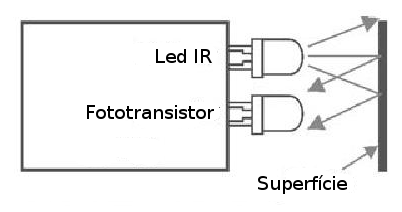
\includegraphics[scale=0.5]{figuras/funcionamento_sensor_obstaculo.png}               
      		\caption{Esquema de funcionamento do sensor de obstáculos por IR (infravermelho).}    
      		\label{img:esquema_sensor_proximidade}                                            
    	\end{figure}     

    	A luz infravermelha gerada pelo LED emissor é refletida pelo objeto onde ela incide e atinge o fototransistor receptor que entra na sua zona de condução. Dependendo da quantidade de luz refletida de volta para o fototransistor, ele detecta o objeto a frente.

    	O sensor de IR escolhido foi o TCRT5000 devido a facilidade de obtenção e baixo custo, além da possibilidade de projetar o sensor ao invés de realizar a compra do módulo pronto, diminuindo mais ainda os custos de produção do robô aspirador. Esse sensor mede até 2.5 centímetros, datasheet disponível em \cite{datasheet_ir}, por isso, caso o sensor detecte que a distância entre ele e o chão supera 2.5 centímetros, o robô irá parar e recalcular sua rota.


  \end{enumerate}
  	

  \subsubsection{Medidor de Bateria}
  \label{sub:Medidor_de_bateria}
    O aspirador de pó não pode ficar sem bateria no meio da execução da limpeza. Para conferir o nível de bateria, será utilizado um comparador de tensão. De forma que, assim que o medidor verificar que o nível da bateria está ficando muito reduzido, um sinal será enviado ao microprocessador que irá interromper o ciclo de limpeza e enviar o robô para a base de carregamento.

    Escolheu-se um circuito comparador que irá comparar a tensão da bateria com até 10 níveis de referência determinados de acordo com a tensão máxima da bateria e o mínimo aceitável para que o robô retorne à base. Essa comparação irá ocorrer por meio de amplificadores operacionais (Amp Op) que irão comparar a tensão que está vindo da bateria com aos níveis de referência. A saída do Amp Op será 1 se o sinal da bateria for maior do que a referência daquele amplificador ou será 0 se o sinal da bateria for menor do que a referência. Para tornar visível o nível da bateria, na saída de cada comparador será adicionado um LED.

    Além de acender ou não os LEDs, cada saída do comparador vai enviar um sinal para o controlador informando o nível da bateria para que ele possa interromper o ciclo de limpeza e enviar o robô para base.

% section instrumentação (end)

\subsection{Hardware para Comunicação}
\label{sub:Hardwar_para_Comunicação}
  A parte de comunicação tem como objetivo coletar informações vindas dos sensores já apresentados, interpreta-las e envia-las para a base onde é feito o intefaceamento com o usuário através de um aplicativo para celular, para essa comunicação serão utilizados 2 microprocessadores, são eles:

    \subsubsection{ATMega 2560}
    Para controlar corretamente as informações obtidas por todos os sensores da parte de instrumentação do projeto é necessário um processador com uma grande quantidade de portas analógicas e digitais, sendo assim utilizaremos o ATMega 2560, que possui as seguintes características:

    \begin{figure}[H]                                                  
      \centering                                                       
      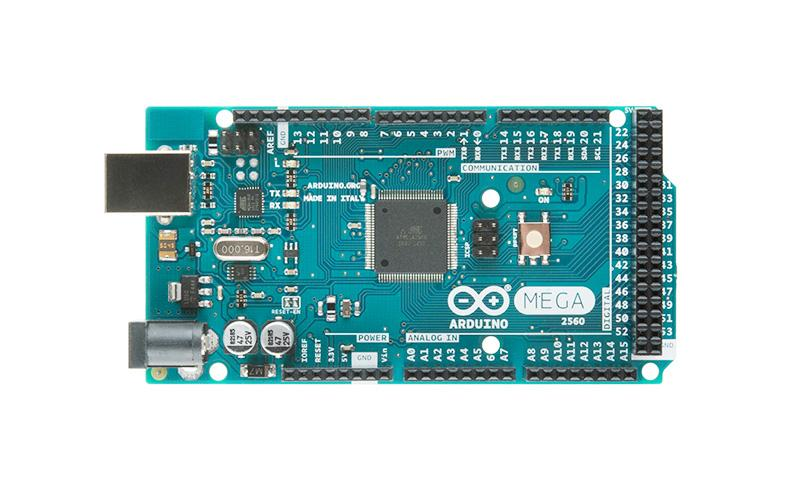
\includegraphics[scale=0.4]{figuras/arduino_mega.png} 
      \caption{Arduíno Mega.}                  
      \label{img:arduino_mega}                                             
    \end{figure}                                                       

 	\textbf{Características:}
    \begin{itemize}
      \item Microcontrolador: ATmega2560
      \item Voltagem de Alimentação: 5V
      \item Voltagem de entrada (recomendada): 7-12V
      \item Voltagem de entrada (limites): 6-20V
      \item Pinos digitais I/O: 54 (dos quais 14 podem ser saídas PWM)
      \item Pinos de entrada analógica: 16
      \item Corrente contínua por pino I/O: 40 mA
      \item Corrente contínua para o pino 3.3V: 50 mA
      \item Memória flash: 256 KB com 4 KB usado para bootloader
      \item SRAM: 8 KB
      \item EEPROM: 4 KB
      \item Velocidade de Clock: 16Mhz
    \end{itemize}
  
  \subsubsection{Módulo de WiFi}
  \label{sub:Modulo_de_wifi}
    Para que o Arduíno possa enviar as informações coletadas para a base é necessário que o mesmo se conecte a rede sem fio, para isso utilizaremos o módulo WiFi ESP8266, ilustrado na figura \ref{img:modulo_wifi}.

  \begin{figure}[H]                                      
    \centering                                           
    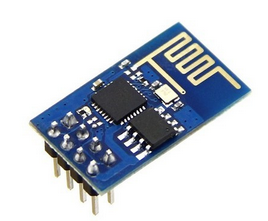
\includegraphics[scale=0.8]{figuras/modulo_wifi.png}
    \caption{Módulo WiFi ESP8266}                              
    \label{img:modulo_wifi}                             
  \end{figure}                                           

  \subsubsection{Raspberry Pi}
  \label{sub:Raspberry}
    Na base para o tráfego de dados, a placa escolhida foi a Raspberry Pi 2 modelo B, este modelo apresenta:

  \begin{figure}[H]                                      
    \centering                                           
    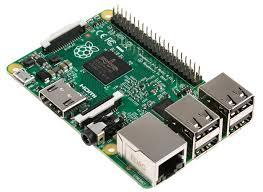
\includegraphics[scale=0.8]{figuras/rasp.jpg} 
    \caption{Raspberry Pi 2 B.}                        
    \label{img:Rasp}                              
  \end{figure}                                           

  \textbf{Especificações:}
  \begin{itemize}                                                     
    \item Chip: Broadcom BCM2836 SoC
    \item Arquitetura: Quad-core ARM Cortex-7
    \item CPU: 900Mhz
    \item Memória RAM: 1GB
    \item GPU Broadcom VideoCore IV
    \item Tensão de operação: Micro USB socket 5V/2ª
    \item Dimensões: 85 x 56 x 17 mm
 \end{itemize}                                                       
  
  Com esse modelo, é possível realizar conexões com a internet e enviar informações ao usuário ou a um banco de dados, por exemplo.

\subsection{Controle} % (fold)
	\label{sub:controle}

		\subsubsection{Sistema de Controle do R2-PI2}

			A parte de controle tem como objetivo desenvolver um sistema capaz de monitorar e controlar a movimentação do aspirador para garantir que os motores sejam devidamente alimentados e juntamente com a parte de instrumentação e comunicação possa garantir a locomoção do robô durante a limpeza sem riscos de colisão com obstáculos.

			O controlador por ora escolhido, ATMega 2560, irá controlar o funcionamento dos motores carrinho e dos sensores. A figura \ref{img:diagrama_sistema_controle} apresenta o diagrama de blocos para o sistema em malha fechada do controle do R2-P12.

			\begin{figure}[H]
				\centering
				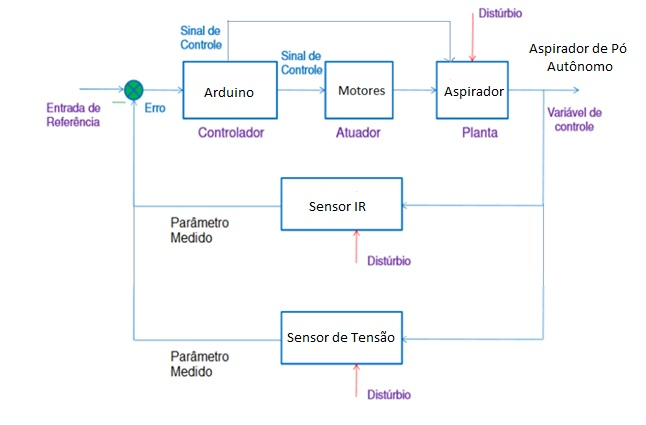
\includegraphics[scale=0.55]{figuras/diagrama_blocos_R2PI2.png}
				\caption{Diagrama de blocos do sistema de controle do R2-PI2. Fonte \cite{mello}.}
				\label{img:diagrama_sistema_controle}
			\end{figure}

			Como mostrado no diagrama, o controlador irá enviar sinais para os motores permitindo que eles sejam ligados ou desligados, fazendo o carrinho se movimentar de acordo com os parâmetros medidos pelos sensores infravermelhos (IR). 

			Serão utilizados sensores IR configurados como detectores de proximidade, na parte frontal  e lateral do aspirador, evitando possíveis colisões com obstáculos em seu caminho, e embaixo dele para evitar vãos como escadas e impedir a queda do robô. Encoderes serão utilizados como controle de posição e também no auxílio da movimentação das rodas quando o aspirador girar para desviar de obstáculos. O monitoramento será contínuo, portanto sempre que houver algum obstáculo ao alcance dos sensores , o controlador enviará um sinal para os motores, impedindo que ocorra choques com objetos no caminho. 

			Será monitorado também, o nível de bateria do robô, quando ele estiver abaixo de um limite que será estabelecido, o controlador enviará um sinal para que o robô possa então retornar para a base e carregar sua bateria. Os componentes envolvidos nessa área são apresentados a seguir.

			\begin{enumerate}
				\item \textbf{Ponte H}:

					Para que se possa controlar a direção e a velocidade dos motores , é necessário que a corrente elétrica possa fluir nas duas direções dentro de sua bobina, gerando campos magnéticos com intensidade e sentidos opostos. A configuração mais utilizada para controlar a corrente nesse projeto é um driver em ponte H (INOUE e OSUKA, 2004).

					O circuito da Ponte H é constituído por quatro transistores que atuam como chave e que, dependendo da configuração do chaveamento, determinam o sentido de rotação dos motores, como pode ser observado na Figura \ref{img:configH}.

					\begin{figure}[H]
						\centering
						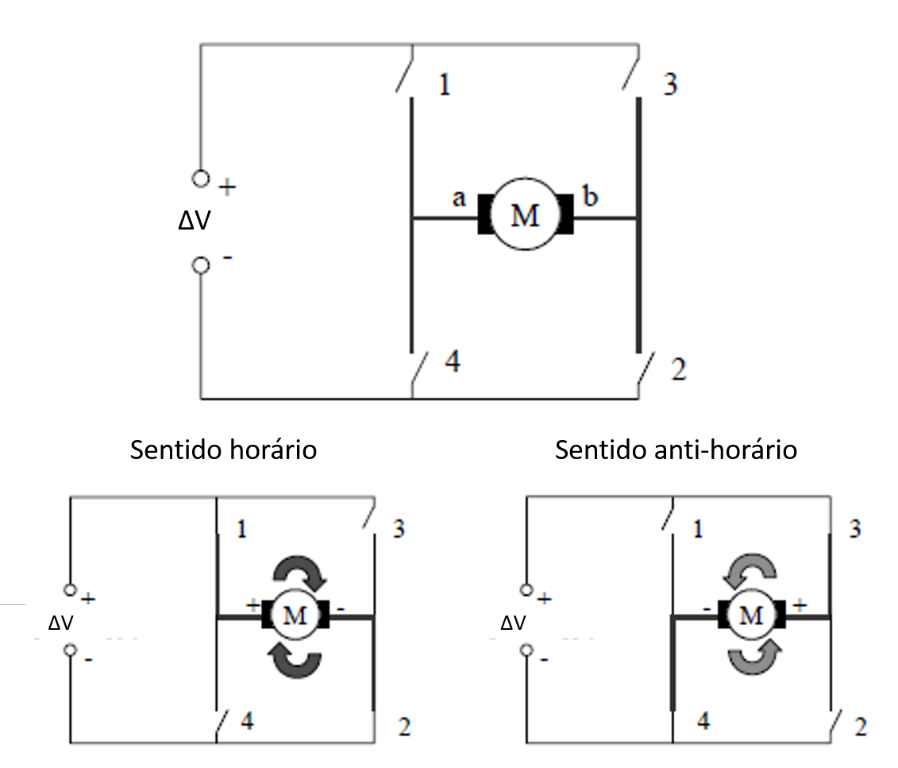
\includegraphics[scale=0.3]{figuras/configH.png}
						\caption{Configurações da Ponte H.}
						\label{img:configH}
					\end{figure}

					A princípio a ponte H escolhida segue o modelo apresentado na Figura \ref{img:modeloH}. 

					\begin{figure}[H]
						\centering
						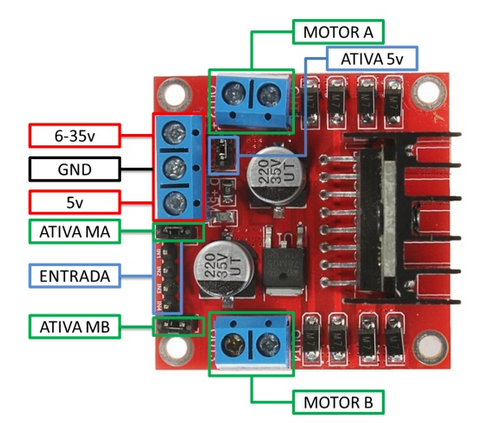
\includegraphics[scale=0.6]{figuras/modeloH.png}
						\caption{Ponte H.}
						\label{img:modeloH}
					\end{figure}

					A escolha foi feita baseando-se na compatibilidade do drive com os motores que devem ser utilizados na movimentação do aspirador.
				\item \textbf{PWM}:

					O controle das velocidades dos motores será feito por meio de chaveamento em frequência constante, gerado pelas saídas digitais do controlador. Para isso utiliza-se o conceito de Pulse-Width Modulation (Modulação por largura de pulso), ou PWM. Com uma onda quadrada com frequência constante e razão cíclica (duty cycle) ajustável , é possível transferir uma determinada quantidade de potência desejável através do valor médio de tensão do sinal \cite{ahmedi}.

					Segundo \cite{ahmedi}, a tensão média de saída é dada por

					\begin{equation}\label{3}
						V_{0} = \frac{Ton.vi}{T}
					\end{equation}
					Onde  é a tensão média de saída,  é o período em segundos em que o sinal fica em nível alto, T o período total do sinal e Vi a tensão de nível alto.

					A potência de saída do sinal pode ser descrita como:

					\begin{equation}
					P = V_{0} . I_{0}
					\end{equation}

					Sendo P a potência de saída,  a tensão de saída e  a corrente de saída. Portanto a partir das equações anteriores pode-se afirmar que:

					\begin{equation}
					V_{0} = Vi . d
					\end{equation}

					onde:

					$d = \frac{Ton}{T}$

					sendo  o duty cycle. A partir da lei de Ohm tem-se então que :

					\begin{equation}
					I_{0} = \frac{d . Vi}{R}
					\end{equation}

					E a potência de saída é dada por:

					\begin{equation}
					P_{0} = \frac{(D . Vi)^{2}}{R}
					\end{equation}

					Considerando-se uma carga totalmente resistiva, pode-se controlar a potência entregue de maneira proporcional a largura de pulso ao quadrado.

					Deve-se observar a frequência de trabalho, para não ultrapassar os limites do hardware de potência em casos onde há carga indutivas, como motores, é necessário pulsar uma frequência que faça a corrente estável para uma mesma largura de pulso, suavizando assim o movimento do motor.

				\item \textbf{Encoder}:

					Os encoders são sensores acoplados no motor para medir a velocidade e posição angular de acordo com a rotação sensoriada por ele. A especificação dos encoders absolutos são medidas em contagem por rotação, CPR, pois de acordo com o número de divisões do encoder e o tamanho da roda conhecem as velocidades, angular e linear, e também a trajetória percorrida \cite{braga}.

					\begin{figure}[H]
						\centering
						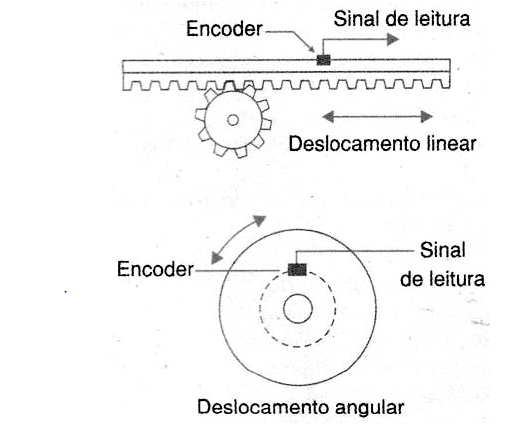
\includegraphics[scale=0.6]{figuras/encoder.png}
						\caption{Sistema de funcionamento de um encoder absoluto.}
						\label{img:encoder}
					\end{figure}

					A posição relativa do aspirador de pó é uma variável muito importante para a navegação e localização que pode ser medida através do uso de encoders [3]. Fixado junto ao motor, o encoder rotacional irá medir a quantidade de rotações do motor e, portanto, possibilitar a obtenção de informações sobre a velocidade angular e posição relativa. 

					Para esse projeto escolheu-se o módulo encoder P17, mostrado na figura \ref{img:modulo_encoder}, que realiza a leitura do sentido do giro e pode ser integrado ao Arduíno.

					\begin{figure}[H]
						\centering
						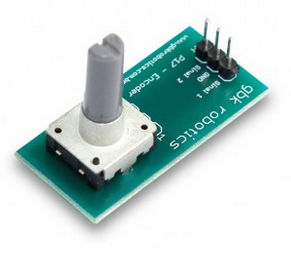
\includegraphics[scale=0.6]{figuras/modulo_encoder.png}
						\caption{Módulo encoder.}
						\label{img:modulo_encoder}
					\end{figure}

			\end{enumerate}



	% subsection controle (end)
% section instrumentação (end)